% ============================================================================
% Chapter 3: Regularization and Generalization Techniques
% ============================================================================
\chapter{Regularization and Generalization Techniques}
\label{ch:regularization}

\noindent\textit{This chapter presents the fundamental techniques for improving the
generalization ability of deep neural networks. We mathematically
derive classical regularization methods (L1, L2, Dropout, Batch
Normalization) and explore modern approaches used in current deep learning
architectures.}\medskip

% ----------------------------------------------------------------------------
\section{Overfitting and underfitting}
\label{sec:overfitting-underfitting}
\index{overfitting}\index{underfitting}

\subsection{Bias-variance decomposition}
\index{bias-variance}

Consider a model $\hat{f}$ trained on a dataset
$\mathcal{D} = \{(x_i, y_i)\}_{i=1}^N$ where $y = f(x) + \epsilon$ with
$\epsilon \sim \mathcal{N}(0, \sigma^2)$.

\begin{mathbox}[title=\textbf{Bias-variance decomposition}]
The mean squared error at a point $x$ decomposes as:
\begin{align}
\E\bigl[(y - \hat{f}(x))^2\bigr]
&= \E\bigl[(f(x) + \epsilon - \hat{f}(x))^2\bigr] \nonumber \\
&= \bigl(f(x) - \E[\hat{f}(x)]\bigr)^2
   + \E\bigl[(\hat{f}(x) - \E[\hat{f}(x)])^2\bigr]
   + \sigma^2 \nonumber \\
&= \underbrace{\text{Bias}^2(\hat{f}(x))}_{\text{systematic error}}
   + \underbrace{\Var(\hat{f}(x))}_{\text{sensitivity to data}}
   + \underbrace{\sigma^2}_{\text{irreducible noise}}
\label{eq:bias-variance}
\end{align}
\end{mathbox}

\begin{definition}[Overfitting]
A model is \textbf{overfitting} when the training error is significantly
lower than the test error:
$\mathcal{L}_{\text{train}} \ll \mathcal{L}_{\text{test}}$. This corresponds
to a high variance in the bias-variance decomposition.
\end{definition}

\begin{definition}[Underfitting]
A model is \textbf{underfitting} when the training error itself is high:
$\mathcal{L}_{\text{train}} \approx \mathcal{L}_{\text{test}} \gg \mathcal{L}^*$.
This corresponds to a high bias.
\end{definition}

\begin{center}
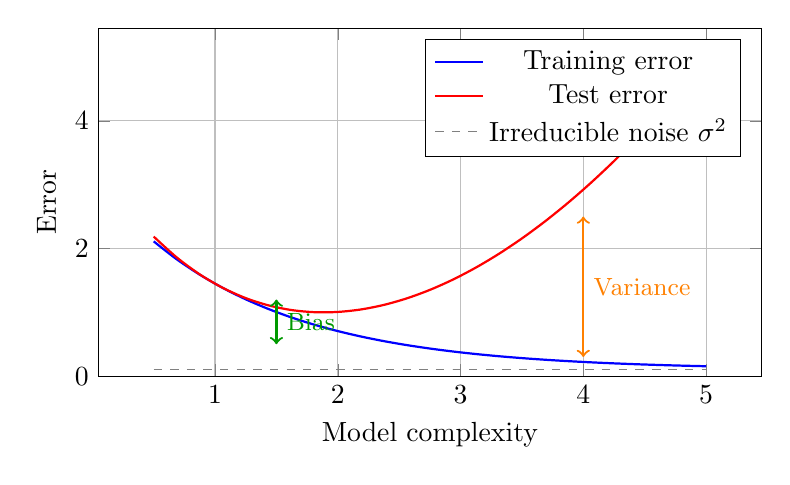
\begin{tikzpicture}
  \begin{axis}[
    width=10cm, height=6cm,
    xlabel={Model complexity},
    ylabel={Error},
    legend pos=north east,
    grid=major,
    ymin=0,
    ]
    \addplot[blue, thick, smooth, domain=0.5:5] {3*exp(-0.8*x) + 0.1};
    \addlegendentry{Training error}
    \addplot[red, thick, smooth, domain=0.5:5] {3*exp(-0.8*x) + 0.3*(x-1)^2 + 0.1};
    \addlegendentry{Test error}
    \addplot[dashed, gray, domain=0.5:5] {0.1};
    \addlegendentry{Irreducible noise $\sigma^2$}
    \draw[<->, thick, green!60!black] (axis cs:1.5,0.5) -- (axis cs:1.5,1.2)
      node[midway, right, font=\small] {Bias};
    \draw[<->, thick, orange] (axis cs:4,0.3) -- (axis cs:4,2.5)
      node[midway, right, font=\small] {Variance};
  \end{axis}
\end{tikzpicture}
\end{center}

% ----------------------------------------------------------------------------
\section{L2 Regularization (Ridge)}
\label{sec:l2-reg}
\index{regularization!L2}\index{Ridge}

\subsection{Formulation}

L2 regularization adds a quadratic penalty on the weights:
\begin{keyformulas}[title=\textbf{L2 regularized cost function}]
\begin{equation}
\tilde{\mathcal{L}}(\theta) = \mathcal{L}(\theta) + \frac{\lambda}{2} \|\theta\|_2^2
= \mathcal{L}(\theta) + \frac{\lambda}{2} \sum_{i} \theta_i^2
\label{eq:l2-cost}
\end{equation}
\end{keyformulas}

\subsection{Gradient derivation}

The gradient of the regularized function is:
\begin{align}
\nabla_\theta \tilde{\mathcal{L}}(\theta)
&= \nabla_\theta \mathcal{L}(\theta) + \lambda \theta
\end{align}

The gradient descent update rule becomes:
\begin{align}
\theta_{t+1} &= \theta_t - \eta \nabla_\theta \tilde{\mathcal{L}}(\theta_t) \nonumber \\
&= \theta_t - \eta \nabla_\theta \mathcal{L}(\theta_t) - \eta \lambda \theta_t \nonumber \\
&= (1 - \eta\lambda)\theta_t - \eta \nabla_\theta \mathcal{L}(\theta_t)
\label{eq:l2-update}
\end{align}

The factor $(1 - \eta\lambda)$ shrinks the weights at each iteration,
hence the name ``weight decay''\index{weight decay}.

\subsection{Geometric interpretation}

\begin{center}
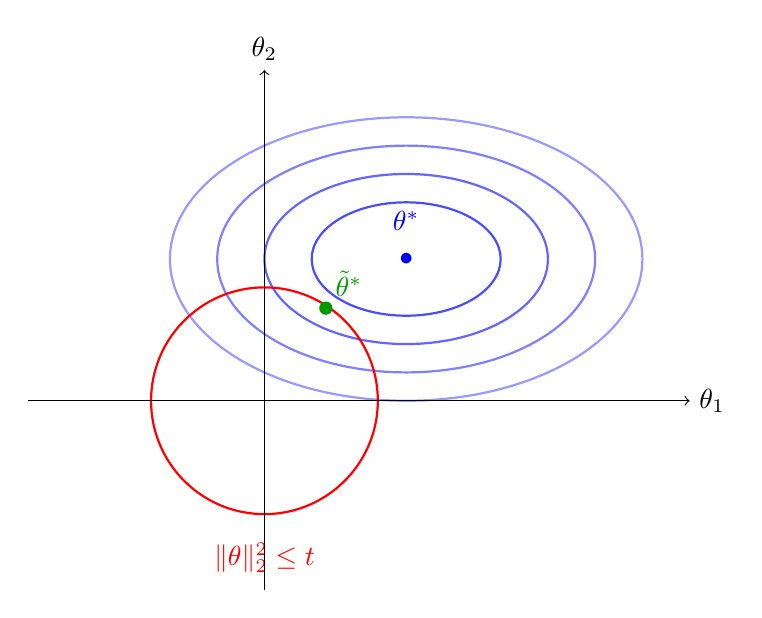
\begin{tikzpicture}[scale=1.2]
  % Loss contours
  \draw[blue!40, thick] (1.5, 1.5) ellipse (2.5 and 1.5);
  \draw[blue!50, thick] (1.5, 1.5) ellipse (2.0 and 1.2);
  \draw[blue!60, thick] (1.5, 1.5) ellipse (1.5 and 0.9);
  \draw[blue!70, thick] (1.5, 1.5) ellipse (1.0 and 0.6);
  \node[blue] at (1.5, 1.5) {$\bullet$};
  \node[blue, above] at (1.5, 1.7) {$\theta^*$};

  % L2 constraint
  \draw[red, thick] (0, 0) circle (1.2);
  \node[red, below] at (0, -1.4) {$\|\theta\|_2^2 \leq t$};

  % Regularized solution
  \fill[green!60!black] (0.65, 0.98) circle (2pt);
  \node[green!60!black, above right] at (0.65, 1.0) {$\tilde{\theta}^*$};

  % Axes
  \draw[->] (-2.5, 0) -- (4.5, 0) node[right] {$\theta_1$};
  \draw[->] (0, -2) -- (0, 3.5) node[above] {$\theta_2$};
\end{tikzpicture}
\end{center}

\begin{intuition}[title=\textbf{Geometric effect of L2}]
L2 regularization constrains the weights to remain within a Euclidean
ball. The regularized solution $\tilde{\theta}^*$ lies at the intersection
of the level curves of $\mathcal{L}$ and the sphere
$\|\theta\|_2 = r$.
\end{intuition}

% ----------------------------------------------------------------------------
\section{L1 Regularization (Lasso)}
\label{sec:l1-reg}
\index{regularization!L1}\index{Lasso}

\begin{keyformulas}[title=\textbf{L1 regularized cost function}]
\begin{equation}
\tilde{\mathcal{L}}(\theta) = \mathcal{L}(\theta) + \lambda \|\theta\|_1
= \mathcal{L}(\theta) + \lambda \sum_{i} |\theta_i|
\label{eq:l1-cost}
\end{equation}
\end{keyformulas}

The subgradient of the L1 penalty is:
\begin{equation}
\frac{\partial}{\partial \theta_i} \lambda |\theta_i| =
\lambda \cdot \text{sign}(\theta_i) =
\begin{cases}
+\lambda & \text{if } \theta_i > 0 \\
-\lambda & \text{if } \theta_i < 0 \\
[-\lambda, +\lambda] & \text{if } \theta_i = 0
\end{cases}
\end{equation}

\begin{remark}[Sparsity of L1]
L1 regularization produces \textbf{sparse} solutions: some weights are
exactly zero. Geometrically, the constraint $\|\theta\|_1 \leq t$ forms
a diamond whose vertices are aligned with the axes, favoring solutions
on the coordinate axes.
\end{remark}

\begin{center}
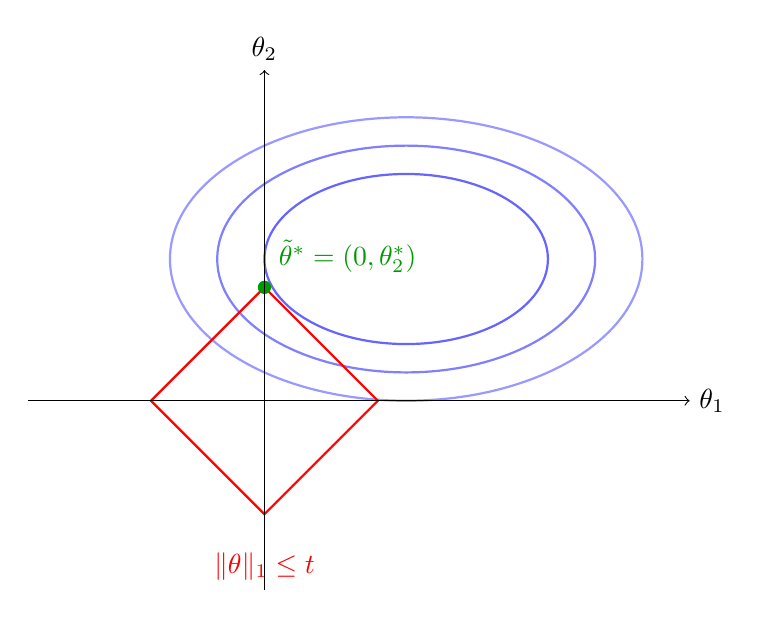
\begin{tikzpicture}[scale=1.2]
  % Loss contours
  \draw[blue!40, thick] (1.5, 1.5) ellipse (2.5 and 1.5);
  \draw[blue!50, thick] (1.5, 1.5) ellipse (2.0 and 1.2);
  \draw[blue!60, thick] (1.5, 1.5) ellipse (1.5 and 0.9);

  % L1 constraint (diamond)
  \draw[red, thick] (1.2, 0) -- (0, 1.2) -- (-1.2, 0) -- (0, -1.2) -- cycle;
  \node[red, below] at (0, -1.5) {$\|\theta\|_1 \leq t$};

  % Sparse solution
  \fill[green!60!black] (0, 1.2) circle (2pt);
  \node[green!60!black, above right] at (0.05, 1.25) {$\tilde{\theta}^* = (0, \theta_2^*)$};

  % Axes
  \draw[->] (-2.5, 0) -- (4.5, 0) node[right] {$\theta_1$};
  \draw[->] (0, -2) -- (0, 3.5) node[above] {$\theta_2$};
\end{tikzpicture}
\end{center}

% ----------------------------------------------------------------------------
\section{Dropout}
\label{sec:dropout}
\index{Dropout}

\subsection{Bernoulli masking}

Dropout \cite{srivastava2014dropout} randomly deactivates a fraction $p$
of neurons during training. For each neuron $j$ in layer $l$, a mask is
sampled:
\begin{equation}
m_j^{(l)} \sim \text{Bernoulli}(1 - p)
\end{equation}

The masked output is:
\begin{equation}
\tilde{h}_j^{(l)} = m_j^{(l)} \cdot h_j^{(l)}
\end{equation}

\subsection{Expectation and inverted Dropout}
\index{Dropout!inverted}

\begin{theorem}[Dropout expectation]
The expectation of the masked output is:
\begin{align}
\E[\tilde{h}_j^{(l)}]
&= \E[m_j^{(l)}] \cdot h_j^{(l)} = (1 - p) \cdot h_j^{(l)}
\end{align}
To maintain the same expectation between training and inference,
\textbf{inverted Dropout} divides by $(1-p)$ during training:
\begin{equation}
\tilde{h}_j^{(l)} = \frac{m_j^{(l)}}{1 - p} \cdot h_j^{(l)}
\label{eq:inverted-dropout}
\end{equation}
Thus $\E[\tilde{h}_j^{(l)}] = h_j^{(l)}$ and no modification is needed
at inference time.
\end{theorem}

\begin{center}
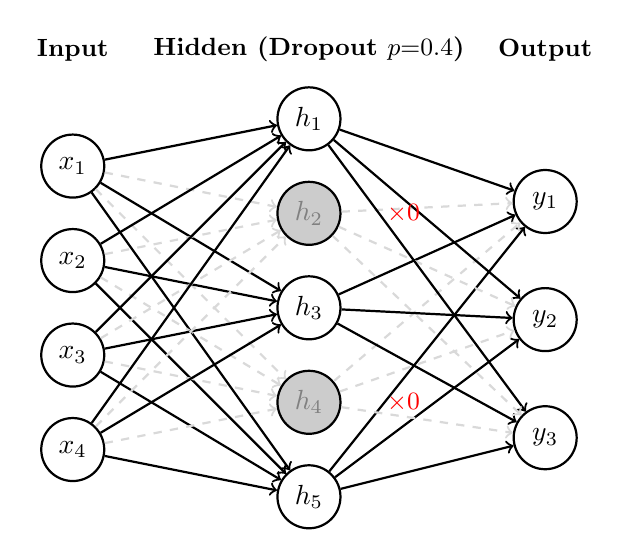
\begin{tikzpicture}[
  neuron/.style={circle, draw, minimum size=8mm, thick},
  dropped/.style={circle, draw, minimum size=8mm, thick, fill=gray!40,
                  text=gray},
  conn/.style={->, thick},
  dropconn/.style={->, thick, gray!30, dashed}
]
  % Input layer
  \foreach \i in {1,2,3,4} {
    \node[neuron] (i\i) at (0, -\i*1.2) {$x_{\i}$};
  }

  % Hidden layer (with dropout)
  \node[neuron] (h1) at (3, -0.6) {$h_1$};
  \node[dropped] (h2) at (3, -1.8) {$h_2$};
  \node[neuron] (h3) at (3, -3.0) {$h_3$};
  \node[dropped] (h4) at (3, -4.2) {$h_4$};
  \node[neuron] (h5) at (3, -5.4) {$h_5$};

  % Output layer
  \foreach \i in {1,2,3} {
    \node[neuron] (o\i) at (6, -\i*1.5 - 0.15) {$y_{\i}$};
  }

  % Input -> hidden connections
  \foreach \i in {1,2,3,4} {
    \foreach \j in {1,3,5} {
      \draw[conn] (i\i) -- (h\j);
    }
    \foreach \j in {2,4} {
      \draw[dropconn] (i\i) -- (h\j);
    }
  }

  % Hidden -> output connections
  \foreach \j in {1,2,3} {
    \foreach \h in {1,3,5} {
      \draw[conn] (h\h) -- (o\j);
    }
    \foreach \h in {2,4} {
      \draw[dropconn] (h\h) -- (o\j);
    }
  }

  % Annotations
  \node[above, font=\small\bfseries] at (0, 0) {Input};
  \node[above, font=\small\bfseries] at (3, 0) {Hidden (Dropout $p{=}0.4$)};
  \node[above, font=\small\bfseries] at (6, 0) {Output};

  \node[red, font=\small] at (4.2, -1.8) {$\times 0$};
  \node[red, font=\small] at (4.2, -4.2) {$\times 0$};
\end{tikzpicture}
\end{center}

% ----------------------------------------------------------------------------
\section{Batch Normalization}
\label{sec:batchnorm}
\index{Batch Normalization}

\subsection{Internal covariate shift problem}
\index{internal covariate shift}

Training deep networks is complicated by the fact that the distribution
of each layer's inputs changes as the weights of preceding layers evolve.
This phenomenon, called \textit{Internal Covariate Shift}
\cite{ioffe2015batch}, slows down convergence.

\subsection{Forward pass}

For a mini-batch $\mathcal{B} = \{x_1, \ldots, x_m\}$:

\begin{keyformulas}[title=\textbf{Batch Normalization -- Forward pass}]
\begin{align}
\mu_{\mathcal{B}} &= \frac{1}{m} \sum_{i=1}^m x_i
\label{eq:bn-mean} \\
\sigma_{\mathcal{B}}^2 &= \frac{1}{m} \sum_{i=1}^m (x_i - \mu_{\mathcal{B}})^2
\label{eq:bn-var} \\
\hat{x}_i &= \frac{x_i - \mu_{\mathcal{B}}}{\sqrt{\sigma_{\mathcal{B}}^2 + \epsilon}}
\label{eq:bn-norm} \\
y_i &= \gamma \hat{x}_i + \beta \equiv \text{BN}_{\gamma, \beta}(x_i)
\label{eq:bn-output}
\end{align}
where $\gamma$ and $\beta$ are learnable parameters, and
$\epsilon > 0$ is a numerical stability term.
\end{keyformulas}

\subsection{Backward pass}

\begin{proposition}[Batch Normalization gradients]
Denoting $\frac{\partial \mathcal{L}}{\partial y_i} = \delta_i$, the
BatchNorm gradients are:
\begin{align}
\frac{\partial \mathcal{L}}{\partial \gamma}
  &= \sum_{i=1}^m \delta_i \hat{x}_i \\
\frac{\partial \mathcal{L}}{\partial \beta}
  &= \sum_{i=1}^m \delta_i \\
\frac{\partial \mathcal{L}}{\partial \hat{x}_i}
  &= \delta_i \cdot \gamma \\
\frac{\partial \mathcal{L}}{\partial \sigma_{\mathcal{B}}^2}
  &= \sum_{i=1}^m \frac{\partial \mathcal{L}}{\partial \hat{x}_i}
     \cdot (x_i - \mu_{\mathcal{B}})
     \cdot \left(-\frac{1}{2}\right)(\sigma_{\mathcal{B}}^2 + \epsilon)^{-3/2} \\
\frac{\partial \mathcal{L}}{\partial \mu_{\mathcal{B}}}
  &= \sum_{i=1}^m \frac{\partial \mathcal{L}}{\partial \hat{x}_i}
     \cdot \frac{-1}{\sqrt{\sigma_{\mathcal{B}}^2 + \epsilon}} \\
\frac{\partial \mathcal{L}}{\partial x_i}
  &= \frac{\partial \mathcal{L}}{\partial \hat{x}_i}
     \cdot \frac{1}{\sqrt{\sigma_{\mathcal{B}}^2 + \epsilon}}
   + \frac{\partial \mathcal{L}}{\partial \sigma_{\mathcal{B}}^2}
     \cdot \frac{2(x_i - \mu_{\mathcal{B}})}{m}
   + \frac{\partial \mathcal{L}}{\partial \mu_{\mathcal{B}}} \cdot \frac{1}{m}
\end{align}
\end{proposition}

% ----------------------------------------------------------------------------
\section{Layer Normalization}
\label{sec:layernorm}
\index{Layer Normalization}

Unlike Batch Normalization which normalizes over the batch dimension,
Layer Normalization \cite{ba2016layer} normalizes over the feature
dimension. For an input $\mathbf{x} \in \R^d$:

\begin{keyformulas}[title=\textbf{Layer Normalization}]
\begin{align}
\mu &= \frac{1}{d} \sum_{j=1}^d x_j, \qquad
\sigma^2 = \frac{1}{d} \sum_{j=1}^d (x_j - \mu)^2 \\
\text{LN}(\mathbf{x}) &= \gamma \odot \frac{\mathbf{x} - \mu}{\sqrt{\sigma^2 + \epsilon}} + \beta
\end{align}
\end{keyformulas}

\begin{remark}[BatchNorm vs LayerNorm]
\begin{itemize}
  \item \textbf{BatchNorm}: normalizes over the batch, each channel independently.
    Mainly used in CNNs (cf.\ Chapter~\ref{ch:cnn}).
  \item \textbf{LayerNorm}: normalizes over the features, each sample
    independently. Used in Transformers
    (cf.\ Chapter~\ref{ch:attention}).
  \item LayerNorm does not depend on batch size and behaves identically
    during training and inference.
\end{itemize}
\end{remark}

% ----------------------------------------------------------------------------
\section{Data augmentation}
\label{sec:data-augmentation}
\index{data augmentation}

\subsection{Classical transformations}

For images: rotations, horizontal flips, random crops, brightness
variations, noise addition.

\subsection{Mixup}
\index{Mixup}

\begin{keyformulas}[title=\textbf{Mixup}]
Given two examples $(x_i, y_i)$ and $(x_j, y_j)$, Mixup
\cite{zhang2018mixup} creates a new example:
\begin{align}
\tilde{x} &= \lambda x_i + (1 - \lambda) x_j \\
\tilde{y} &= \lambda y_i + (1 - \lambda) y_j
\end{align}
where $\lambda \sim \text{Beta}(\alpha, \alpha)$ with $\alpha > 0$.
\end{keyformulas}

\subsection{CutMix}
\index{CutMix}

\begin{keyformulas}[title=\textbf{CutMix}]
CutMix \cite{yun2019cutmix} replaces a rectangular region of $x_i$ with
the corresponding region of $x_j$:
\begin{align}
\tilde{x} &= \mathbf{M} \odot x_i + (1 - \mathbf{M}) \odot x_j \\
\tilde{y} &= \lambda y_i + (1 - \lambda) y_j
\end{align}
where $\mathbf{M} \in \{0, 1\}^{H \times W}$ is a binary mask and
$\lambda = 1 - \frac{r_w \cdot r_h}{W \cdot H}$ represents the proportion
of the original image.
\end{keyformulas}

% ----------------------------------------------------------------------------
\section{Early Stopping}
\label{sec:early-stopping}
\index{early stopping}

\begin{definition}[Early stopping]
Early stopping consists of halting training when the validation error
stops decreasing for a predefined number of epochs
(``patience'').
\end{definition}

\begin{theorem}[Equivalence with L2 regularization]
For a quadratic linear model with gradient descent, stopping at
iteration $T$ is approximately equivalent to L2 regularization with
$\lambda \approx \frac{1}{\eta T}$, where $\eta$ is the learning rate.

\textbf{Proof.} Let $\mathcal{L}(\theta) = \frac{1}{2}(\theta - \theta^*)^\top H (\theta - \theta^*)$
with $H$ the Hessian. Starting from $\theta_0 = 0$, after $T$ iterations:
\begin{equation}
\theta_T = (I - (I - \eta H)^T) \theta^*
\end{equation}
For L2 regularization, the solution is
$\tilde{\theta} = (H + \lambda I)^{-1} H \theta^*$.
Using the spectral decomposition $H = Q \Lambda Q^\top$, one can show
that the two solutions coincide when
$1 - (1 - \eta \lambda_i)^T \approx \frac{\lambda_i}{\lambda_i + 1/(\eta T)}$.
\end{theorem}

% ----------------------------------------------------------------------------
\section{Weight Decay vs L2 in Adam}
\label{sec:weight-decay-adam}
\index{weight decay!Adam}\index{AdamW}

\begin{warning}[title=\textbf{Crucial difference}]
Weight decay and L2 regularization are \textbf{not equivalent} for
adaptive optimizers like Adam!
\end{warning}

\subsection{L2 regularization in Adam}

With L2 in Adam, the modified gradient is $g_t = \nabla \mathcal{L}(\theta_t) + \lambda \theta_t$.
This gradient is then normalized by Adam's moments:
\begin{align}
m_t &= \beta_1 m_{t-1} + (1 - \beta_1)(g_t + \lambda \theta_t) \\
v_t &= \beta_2 v_{t-1} + (1 - \beta_2)(g_t + \lambda \theta_t)^2 \\
\theta_{t+1} &= \theta_t - \eta \frac{\hat{m}_t}{\sqrt{\hat{v}_t} + \epsilon}
\end{align}

The regularization term $\lambda \theta_t$ is \textbf{attenuated} by
the adaptive normalization $\frac{1}{\sqrt{\hat{v}_t} + \epsilon}$.

\subsection{AdamW: Decoupled Weight Decay}

AdamW \cite{loshchilov2019decoupled} applies weight decay directly:
\begin{keyformulas}[title=\textbf{AdamW}]
\begin{align}
m_t &= \beta_1 m_{t-1} + (1 - \beta_1) g_t \\
v_t &= \beta_2 v_{t-1} + (1 - \beta_2) g_t^2 \\
\theta_{t+1} &= (1 - \eta\lambda)\theta_t
               - \eta \frac{\hat{m}_t}{\sqrt{\hat{v}_t} + \epsilon}
\end{align}
\end{keyformulas}

\begin{bestpractice}[title=\textbf{Use AdamW}]
In practice, \textbf{AdamW} (decoupled weight decay) should be
preferred over Adam with L2 regularization. AdamW is the standard
optimizer for modern Transformers.
\end{bestpractice}

% ----------------------------------------------------------------------------
\section{PyTorch implementation}
\label{sec:reg-pytorch}

\begin{codeblock}[title=\textbf{Complete regularized training loop}]
\begin{minted}{python}
import torch
import torch.nn as nn
import torch.optim as optim
from torch.utils.data import DataLoader
from torchvision import datasets, transforms

# --- Model with Dropout and BatchNorm ---
class RegularizedNet(nn.Module):
    def __init__(self, input_dim=784, hidden_dim=256,
                 num_classes=10, dropout_rate=0.5):
        super().__init__()
        self.layers = nn.Sequential(
            nn.Linear(input_dim, hidden_dim),
            nn.BatchNorm1d(hidden_dim),
            nn.ReLU(),
            nn.Dropout(p=dropout_rate),
            nn.Linear(hidden_dim, hidden_dim),
            nn.BatchNorm1d(hidden_dim),
            nn.ReLU(),
            nn.Dropout(p=dropout_rate),
            nn.Linear(hidden_dim, num_classes)
        )

    def forward(self, x):
        return self.layers(x.view(x.size(0), -1))

# --- Configuration ---
device = torch.device('cuda' if torch.cuda.is_available() else 'cpu')
model = RegularizedNet(dropout_rate=0.3).to(device)

# AdamW with decoupled weight decay
optimizer = optim.AdamW(model.parameters(), lr=1e-3,
                        weight_decay=1e-4)
criterion = nn.CrossEntropyLoss(label_smoothing=0.1)
scheduler = optim.lr_scheduler.CosineAnnealingLR(optimizer, T_max=50)

# --- Data augmentation ---
transform_train = transforms.Compose([
    transforms.RandomRotation(10),
    transforms.RandomAffine(0, translate=(0.1, 0.1)),
    transforms.ToTensor(),
    transforms.Normalize((0.1307,), (0.3081,))
])

train_dataset = datasets.MNIST(root='./data', train=True,
                               transform=transform_train, download=True)
train_loader = DataLoader(train_dataset, batch_size=128, shuffle=True)
val_loader = DataLoader(
    datasets.MNIST(root='./data', train=False,
                   transform=transforms.Compose([
                       transforms.ToTensor(),
                       transforms.Normalize((0.1307,), (0.3081,))
                   ])),
    batch_size=256, shuffle=False
)

# --- Early Stopping ---
class EarlyStopping:
    def __init__(self, patience=10, min_delta=1e-4):
        self.patience = patience
        self.min_delta = min_delta
        self.counter = 0
        self.best_loss = float('inf')
        self.should_stop = False

    def __call__(self, val_loss):
        if val_loss < self.best_loss - self.min_delta:
            self.best_loss = val_loss
            self.counter = 0
        else:
            self.counter += 1
            if self.counter >= self.patience:
                self.should_stop = True

early_stopping = EarlyStopping(patience=10)

# --- Training loop ---
for epoch in range(50):
    model.train()
    train_loss = 0.0
    for inputs, targets in train_loader:
        inputs, targets = inputs.to(device), targets.to(device)
        optimizer.zero_grad()
        outputs = model(inputs)
        loss = criterion(outputs, targets)
        loss.backward()
        torch.nn.utils.clip_grad_norm_(model.parameters(), max_norm=1.0)
        optimizer.step()
        train_loss += loss.item()

    # Validation
    model.eval()
    val_loss = 0.0
    correct = 0
    with torch.no_grad():
        for inputs, targets in val_loader:
            inputs, targets = inputs.to(device), targets.to(device)
            outputs = model(inputs)
            val_loss += criterion(outputs, targets).item()
            correct += (outputs.argmax(1) == targets).sum().item()

    val_loss /= len(val_loader)
    accuracy = correct / len(val_loader.dataset)
    scheduler.step()

    print(f"Epoch {epoch+1}: train_loss={train_loss/len(train_loader):.4f}, "
          f"val_loss={val_loss:.4f}, accuracy={accuracy:.4f}")

    early_stopping(val_loss)
    if early_stopping.should_stop:
        print("Early stopping triggered.")
        break
\end{minted}
\end{codeblock}

% ----------------------------------------------------------------------------
\section{Ablation study}
\label{sec:reg-ablation}

\begin{codeblock}[title=\textbf{Ablation study: Dropout rate and Weight Decay}]
\begin{minted}{python}
import itertools
import pandas as pd

results = []
dropout_rates = [0.0, 0.1, 0.3, 0.5, 0.7]
weight_decays = [0.0, 1e-5, 1e-4, 1e-3, 1e-2]

for dr, wd in itertools.product(dropout_rates, weight_decays):
    model = RegularizedNet(dropout_rate=dr).to(device)
    optimizer = optim.AdamW(model.parameters(), lr=1e-3,
                            weight_decay=wd)
    # Train for 20 epochs (simplified)
    for epoch in range(20):
        model.train()
        for inputs, targets in train_loader:
            inputs, targets = inputs.to(device), targets.to(device)
            optimizer.zero_grad()
            loss = criterion(model(inputs), targets)
            loss.backward()
            optimizer.step()

    # Evaluate
    model.eval()
    correct = 0
    with torch.no_grad():
        for inputs, targets in val_loader:
            inputs, targets = inputs.to(device), targets.to(device)
            correct += (model(inputs).argmax(1) == targets).sum().item()
    acc = correct / len(val_loader.dataset)
    results.append({'dropout': dr, 'weight_decay': wd, 'accuracy': acc})

df = pd.DataFrame(results)
pivot = df.pivot(index='dropout', columns='weight_decay', values='accuracy')
print(pivot.to_string(float_format='{:.4f}'.format))
\end{minted}
\end{codeblock}

\begin{codeoutput}
\begin{verbatim}
weight_decay    0.0     1e-05   0.0001  0.001   0.01
dropout
0.0           0.9812  0.9821  0.9835  0.9801  0.9754
0.1           0.9838  0.9842  0.9851  0.9828  0.9773
0.3           0.9845  0.9849  0.9856  0.9839  0.9790
0.5           0.9831  0.9835  0.9843  0.9821  0.9779
0.7           0.9762  0.9770  0.9778  0.9755  0.9701
\end{verbatim}
\end{codeoutput}

\begin{remark}[Observations]
\begin{itemize}
  \item Dropout at $p=0.3$ with weight decay $\lambda=10^{-4}$ yields the
    best results on MNIST.
  \item Too high a Dropout ($p=0.7$) degrades performance by overly
    limiting the network's capacity.
  \item Weight decay at $10^{-2}$ is too aggressive and hurts performance
    across all Dropout rates.
\end{itemize}
\end{remark}

% ----------------------------------------------------------------------------
\section{State-of-the-art techniques}
\label{sec:reg-sota}

\begin{sota}[title=\textbf{Modern regularization techniques}]
\begin{description}
  \item[Stochastic Depth] \cite{huang2016deep}: randomly deactivates
    entire residual blocks (see Chapter~\ref{ch:cnn}). Each block
    $l$ has a survival probability $p_l = 1 - \frac{l}{L}(1 - p_L)$.
    \index{Stochastic Depth}

  \item[DropPath]: variant of Stochastic Depth applied per path
    in multi-branch architectures. Used in EfficientNet and
    Vision Transformers.
    \index{DropPath}

  \item[Label Smoothing] \cite{szegedy2016rethinking}: replaces one-hot
    targets with:
    \begin{equation}
      y_k^{\text{LS}} = (1 - \alpha) y_k + \frac{\alpha}{K}
    \end{equation}
    where $K$ is the number of classes and $\alpha \in [0, 1]$ is the
    smoothing parameter (typically $\alpha = 0.1$).
    \index{Label Smoothing}

  \item[R-Drop] \cite{wu2021r}: minimizes the KL divergence between two
    forward passes with different Dropout:
    \begin{equation}
      \mathcal{L}_{\text{R-Drop}} = \mathcal{L}_{\text{CE}}
        + \alpha \cdot \frac{1}{2}\bigl(\KL(p_1 \| p_2) + \KL(p_2 \| p_1)\bigr)
    \end{equation}
    \index{R-Drop}
\end{description}
\end{sota}

% ----------------------------------------------------------------------------
\section{Exercises}
\label{sec:reg-exercises}

\begin{exercise}[Bias-variance decomposition \hfill $\bigstar$]
Let $f(x) = \sin(\pi x)$ and $\hat{f}$ be a polynomial of degree $d$ fitted
on $N = 10$ noisy points ($\sigma = 0.3$).
\begin{enumerate}
  \item Prove the bias-variance decomposition (Equation~\ref{eq:bias-variance}).
  \item Simulate in Python the error for $d \in \{1, 3, 5, 9, 15\}$ over 100
    datasets. Plot bias$^2$, variance, and total error.
  \item Which degree offers the best trade-off?
\end{enumerate}
\end{exercise}

\begin{exercise}[Elastic Net regularization \hfill $\bigstar\bigstar$]
Elastic Net combines L1 and L2:
$\Omega(\theta) = \alpha \|\theta\|_1 + \frac{1-\alpha}{2}\|\theta\|_2^2$.
\begin{enumerate}
  \item Derive the update rule with proximal gradient descent for the L1 part.
  \item Implement this regularization in PyTorch by manually modifying
    the gradients.
  \item Compare the solutions with L1 alone, L2 alone, and Elastic Net on a
    linear regression problem with $p = 100$ variables of which 10 are
    relevant.
\end{enumerate}
\end{exercise}

\begin{exercise}[Dropout as a model ensemble \hfill $\bigstar\bigstar$]
\begin{enumerate}
  \item Show that a network with Dropout at rate $p$ on $n$ units
    implicitly implements an ensemble of $2^n$ sub-networks.
  \item For a single hidden layer network ($d$ units) with Dropout,
    derive the geometric mean approximation of the weight
    $W_{\text{test}} = (1-p) W_{\text{train}}$.
  \item Implement MC-Dropout (Monte Carlo Dropout) to estimate
    predictive uncertainty and compare with standard Dropout on a
    regression problem.
\end{enumerate}
\end{exercise}

\begin{exercise}[BatchNorm implementation from scratch \hfill $\bigstar\bigstar\bigstar$]
\begin{enumerate}
  \item Implement complete Batch Normalization (forward and backward)
    without using \texttt{nn.BatchNorm1d}.
  \item Verify the backward correctness with \texttt{torch.autograd.gradcheck}.
  \item Compare convergence speed with and without BatchNorm on CIFAR-10.
  \item Study the effect of batch size on BatchNorm stability
    (batch sizes: 4, 16, 64, 256).
\end{enumerate}
\end{exercise}

\begin{exercise}[AdamW vs Adam + L2 \hfill $\bigstar\bigstar\bigstar$]
\begin{enumerate}
  \item Formally prove that for SGD, weight decay and L2 are
    equivalent with $\lambda_{\text{wd}} = \frac{\lambda_{L2}}{\eta}$.
  \item Show that this equivalence breaks down for Adam by exhibiting
    an analytical counterexample (2-parameter model with very
    different gradient magnitudes).
  \item Train a (small) Transformer model with Adam+L2 and AdamW,
    varying the regularization coefficient. Plot the generalization
    curves and compare.
\end{enumerate}
\end{exercise}
